\documentclass[12pt]{article}
% Margin fixes
\oddsidemargin -0.5in
\evensidemargin -0.5in
\textwidth 7.25in
\topmargin 0.0in

\headheight 0.0pt
\headsep 0.0pt
\voffset 0.0pt
\textheight = 9.0in
\usepackage{amsmath,amssymb,graphicx,float}

\title{Frank-Hertz}
\author{Nathan Grouse\\Lisa Tran}

\newcommand{\eV}{\text{eV}}
\newcommand{\V}{\text{V}}
\newcommand{\A}{\text{A}}

% Start the document!
\newcommand{\documentname}{\textsl{Article}}
\begin{document}
\maketitle

\section{Introduction}
\indent \indent Electrons are accelerated through a tubed filled with mercury atoms by a steadily increasing voltage. The collisions between the electrons and mercury atoms are elastic as long as the electron energy remains below 4.9 eV - this is the energy of the first excited state of Mercury. As the electron energy rises above 4.9 eV, the electrons which undergo inelastic collisions are unable to make it past a retarding voltage $U_3$,
resulting in a sudden drop in the anode current. As the driving voltage is increased more, the anode current increases until the electron energy rises above the energy of the second excited state of Mercury. The goals of this experiment are to reproduce the results obtain by James Franck and Gustav Hertz, and to build physical intuition of quantum effects and particle interactions at the atomic level.

\subsection{Apparatus}
\indent \indent A cathode is inserted in a hollowed out copper tube and indirectly heated by a filament which is heated directly by a voltage source. Inside the cathode there are a cathode, two voltage grids, and an anode. The entire apparatus is also heated by a small oven. An oscilloscope is used to adjust the voltages before recording data.

\section{Data}
\begin{figure}[H]
\centering
\hspace{-0.0in}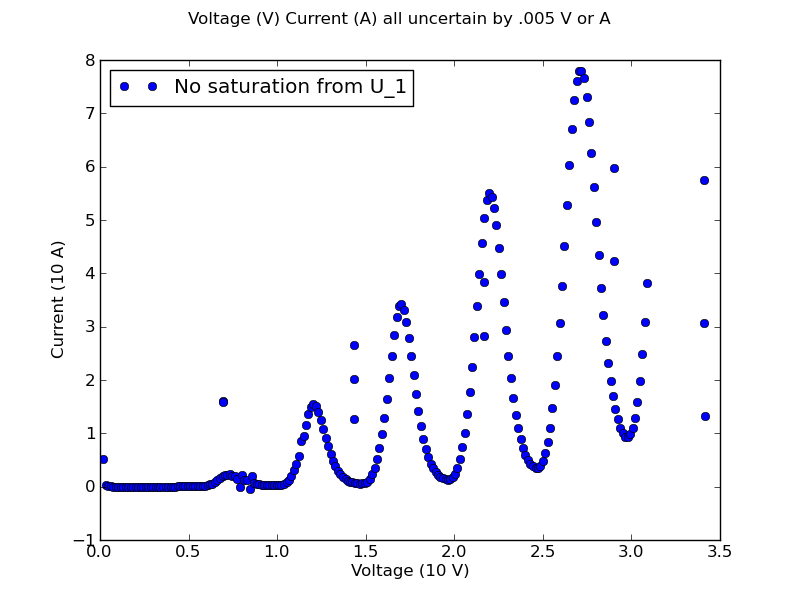
\includegraphics[scale=0.60]{Plot1.png}
\caption{No Saturation \label{fig:setup}}
\end{figure}

\begin{figure}[H]
\centering
\hspace{-0.0in}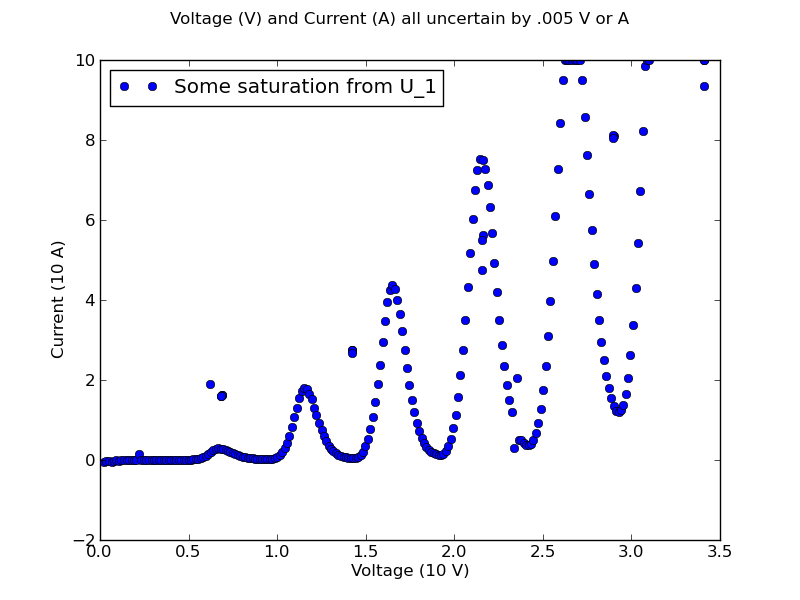
\includegraphics[scale=0.60]{Plot2.png}
\caption{Some Saturation \label{fig:setup}}
\end{figure}

\section{Calculations}
\indent \indent
\[(U_1 + U_2) - U_3 = 4.9 \,\V\]
Where $U_1$ is the voltage across the control grid, $U_2$ is the acceleration grid, and $U_3$ is the retarding voltage. Theoretically this should be the case.
\[ U_1 = 1 \, \V \]
\[U_2 = 7.32 \, \V \]
\[ U_3 = 3.5 \, \V \]
Actual values yield:
\[(U_1 + U_2) - U_3 = 4.82 \,\V\]

\section{Error Analysis}
\indent \indent Uncertainty in Voltage and Current was determined from the SWS data. The data gave values out to 3 decimal places, meaning it rounded somewhere around $\pm .05$ of the respective value. If we wish to find how uncertainty propogates in our evaluation of the energy of the first excited state, simply add the uncertainties in each voltage in quadrature:
\[\delta E = \sqrt{(\delta U_1)^2 + (\delta U_2)^2 + (\delta U_3)^2} \]
Percent Error:
\[\frac{|4.9 - 4.82|}{4.9} = 1.6 \% \]

\section{Conclusion}
\indent \indent The number I obtained is both reasonable and consistent with the accepted value. I did see what I expected to see, with the small exception of the current peaks flattening out on the oscilloscope at higher voltages. Originally, I didn't understand the orientation of the voltage grids in this cathode ray tube. After examining figure 1 at the end of the manual and talking through it with you, I have a clear understanding. Electrons move from the axis of the cylinder to the outer surface and can only make it to the anode if they have enough energy to make it past the retarding voltage $U_3$.

\section{Questions}
1. Indirectly heating the cathode through a copper barrier is desirable because it results in a more even heating of the tube. \\
2. At higher temperatuers, mercury's electrons and random thermal electrons in the tube do a better job of keeping Mercury in an excited state. Slowly coming down from a higher temperature allows smoother discharge from the excited states by slowly increasing the rate of de-excitation. \\
3. If the oven temperature was too high the tube would be destroyed. Its components would melt and crack. \\
4. A peak would not occur at $(U_1 + U_2) = 4.9$ because the electrons would not have enough energy to overcome the retarding voltage $U_3$ after undergoing inelastic collisions with the mercury.

\end{document}